%---------------------------------------------------------------------
% This file provides a skeleton UCL DIS CDT report.
% \pdfinclusioncopyfonts=1
% This command may be needed in order to get \ell in PDF plots to appear. Found in
% https://tex.stackexchange.com/questions/322010/pdflatex-glyph-undefined-symbols-disappear-from-included-pdf
%---------------------------------------------------------------------
% Specify where LaTeX style files can be found.
\newcommand*{\DISCDTLATEXPATH}{latex/}
% Use this variant if the files are in a central location, e.g. $HOME/texmf.
%---------------------------------------------------------------------

\documentclass[NOTE, disdraft=true, UKenglish]{\DISCDTLATEXPATH UCLCDTDISdoc}
% The language of the document must be set: usually UKenglish or USenglish.
% british and american also work!
% Commonly used options:
%  cdtdraft=true|false   This document is a UCL CDT DIS draft.
%  paper=a4|letter       Set paper size to A4 (default) or letter.

%--------------------------------------------------------------------- 
% Add you own definitions here (file dis-gp-defs.sty).
%\usepackage{dis-gp-defs}
%---------------------------------------------------------------------


%--------------------------------------------------------------------- 
% Files with references for use with biblatex.
% Note that biber gives an error if it finds empty bib files.
\usepackage{biblatex} % uncomment if use addbibresource command
\addbibresource{template/PNET_project.bib}
%--------------------------------------------------------------------- 

% Paths for figures - do not forget the / at the end of the directory name.
\graphicspath{{logos/}{figures/}}


%---------------------------------------------------------------------
% Generic document information
%---------------------------------------------------------------------
% Title, abstract and document 
%-------------------------------------------------------------------------
% This file contains the title, author and abstract.
% It also contains all relevant document numbers if needed.
%-------------------------------------------------------------------------

% Partner Logo
% put the name of the logo image file found in graphics path
\DISPartnerLogo{logos/UCL_purple.png}


% Title
\DISTitle{Improving radiosensitivity predictions of brain cells using a biologically informed neural network}

% Draft version:
% If given, adds draft version on front page, a 'DRAFT' box on top of each other page, 
% and line numbers.
% Comment or remove in final version.
\DISVersion{0}

% Abstract - % directly after { is important for correct indentation
\DISAbstract{%
  One of the current most effective treatments for brain tumor's is radiotherapy. However, this has the side-effect of damaging healthy cells with potentially severe consequences. Improvements in radiotherapy treatment such as proton therapy allow a more spatially localized treatment. However, the sensitivity of different cell types to radioactivity is not currently well modeled. We present a method for predicting the radio-sensitivity of a cell based on its genetic content using a biologically informed neural network. We compare the use of different data features for training this model, different network architecture and develop a procedure for transfer learning, where drug response data is incorporated into the model training. We compare the model performance using a cross-validation procedure ensuring unbiased performance estimates with faithful uncertainty estimates. We find ...
}


% Authors and list of contributors to the analysis
\usepackage{authblk}
\author[a]{Toby Dixon}
\author[a]{Dakshesh Kololgi}
\author[b]{Jason Ran}

\affil[a]{University College London}


% DIS reference code if ever used
\DISRefCode{UCLCDTDIS-2024-XX}

% Author and title for the PDF file
\hypersetup{pdftitle={UCL CDT DIS Document},pdfauthor={The UCL CDT DIS}}

%---------------------------------------------------------------------
% Content
%---------------------------------------------------------------------
\begin{document}

\maketitle

\tableofcontents

\clearpage


%---------------------------------------------------------------------
\newpage
%---------------------------------------------------------------------

\newpage
%---------------------------------------------------------------------
\section{Introduction}
\label{sec:introduction}
Cancer is one of the largest causes of mortality in developed countries. This has lead to intensive research into cancer treatments. One of the most promising is radiotherapy, in this treatment malignant tumors are treated with ionizing radiation (typically X-rays). However, this treatments still induce a significant amount of damage to healthy cells which can have severe effects.
Developments in radiotherapy such as proton beam therapy \cite{proton_beam} allow for more spatially targeted treatments based on a patients particular gene profile. This opens up the possibility of optimizing treatments to avoid regions expected to have high radiation sensitivity. In addition, developments in genetic sequencing mean that large number of genetic information is available to base radio-sensitivity predictions on. It is relatively challenging to measure the radiation response of cells, this leads to only very small datasets to be available. This leads to a situation where a large number of features are available for each data sample but only a small number of samples which can easily lead to overfitting.
\\ \indent 
Predicting radio-sensitivity based on genetic data has been investigated using some classical approaches such as least squares regression \cite{SCOTT2017202}. In addition, machine learning methods could be employed as in \cite{speers2015development}. In general these methods require heavy regularization due to the small available datasets.
\\ \indent  In this work we develop a radio-sensitivity predictor using a biologically informed neural network (BNN) \cite{review,review_2}. This type of model consists of a sparse neural network where the connections represent known biologically processes, which are compiled in genetic databases \cite{Reactome,gene_ontology}. This has the advantage that the number of fitted parameters is much smaller, preventing over-fitting and the outputs of the model can be interpreted potentially leading to biological insights.
\\ \indent 
The model we will use called P-NET\cite{elmarakeby_biologically_2021}, was developed for the classification of prostate cancer cells. This model has been adapted for radio-sensitivity predictions \cite{cosmin_thesis}. In addition, we have explored applying transfer learning \cite{transfer} to radio-sensitivity predictions. In this approach a model can be trained using information from drug response data, which is more readily available.
\\ \indent 
This report describes a systematic comparison of P-NET used for radiation predictions using different data-types and network architectures. 
In \ref{sec:data} we describe the genetic data used for this study, in \ref{sec:method} we describe in more detail the model and our framework for model comparisons. Finally, in section \ref{sec:results} we describe the results. The outlook for future studies is described in \ref{sec:conclusion}.
 
%\input{introduction}
%---------------------------------------------------------------------
\section{Data}
\label{sec:data}
{\color{red}Toby: I think what we should do here is describe the available datasets (where they come from, the size the features), and make some nice plots to show the distributions in data etc.}
\\
For this work, we use genomic data as predictors. This type of information is contained within a cell and enables its growth and reproduction. It is characterised by DNA (deoxyribonucleic acid), RNA (ribonucleic acid), and proteins. We focus on gene expression data


data from the CCLE (full name+ \ref{}) database. This consists of measurements of the radio-sensitivity of 511 cell lines along with their genetic sequence. The radio-sensitivity is characterized by the area under the dose-response curve (AUC). This is a relatively expensive measure requiring irradiation of cells with known doses of radiation. This limits the size of the available dataset. 
\\ \indent However, advances in genetic sequencing \ref{} mean that for each cell line, there is a large amount of genetic information available. Thus the dataset available has a large number of features but very few data points. This situation can easily lead to over-fitting \ref{}. We focus on 3 genetic features. Gene expression, copy number violation, and mutations.

\section{Methods}
\label{sec:method}
For this work, we employ a biologically informed neural network to predict the radio-sensitivity. This is based on our adaptation of P-NET \cite{cosmin_thesis}. A typical dense neural network has millions of connections, and thus weights to tune. This can easily lead to over-fitting where the model predicts well on the training dataset but not on unseen data. A solution to this is to encode some prior knowledge into the model's architecture. In this way, we create a sparse network where the connections represent known biological pathways.

\subsection{Network architecture}
P-NET is a feed-forward Biologically Informed Neural Network originally developed to classify prostate cancer tumours into being either primary or metastatic types. P-NET consists of six layers arranged such that the constituent neurons encode the hierarchical manner of the Reactome or Gene Ontology bio-informatics databases. Each successive layer encodes increasingly more complex biological processes. This was implemented by selectively connecting neurons between layers depending on the hierarchies in Reactome or Gene Ontology.\\

This work significantly re-structured P-NET to enable connections between layers to be informed by Gene Ontology in addition to Reactome. We draw from Kuenzi et al.'s implementation of the DrugCell Deep Learning model that, in analogy with P-NET, utilises Gene Ontology for cancer cell drug sensitivity prediction \cite{kuenzi_predicting_2020}.

\begin{figure}
    \centering
    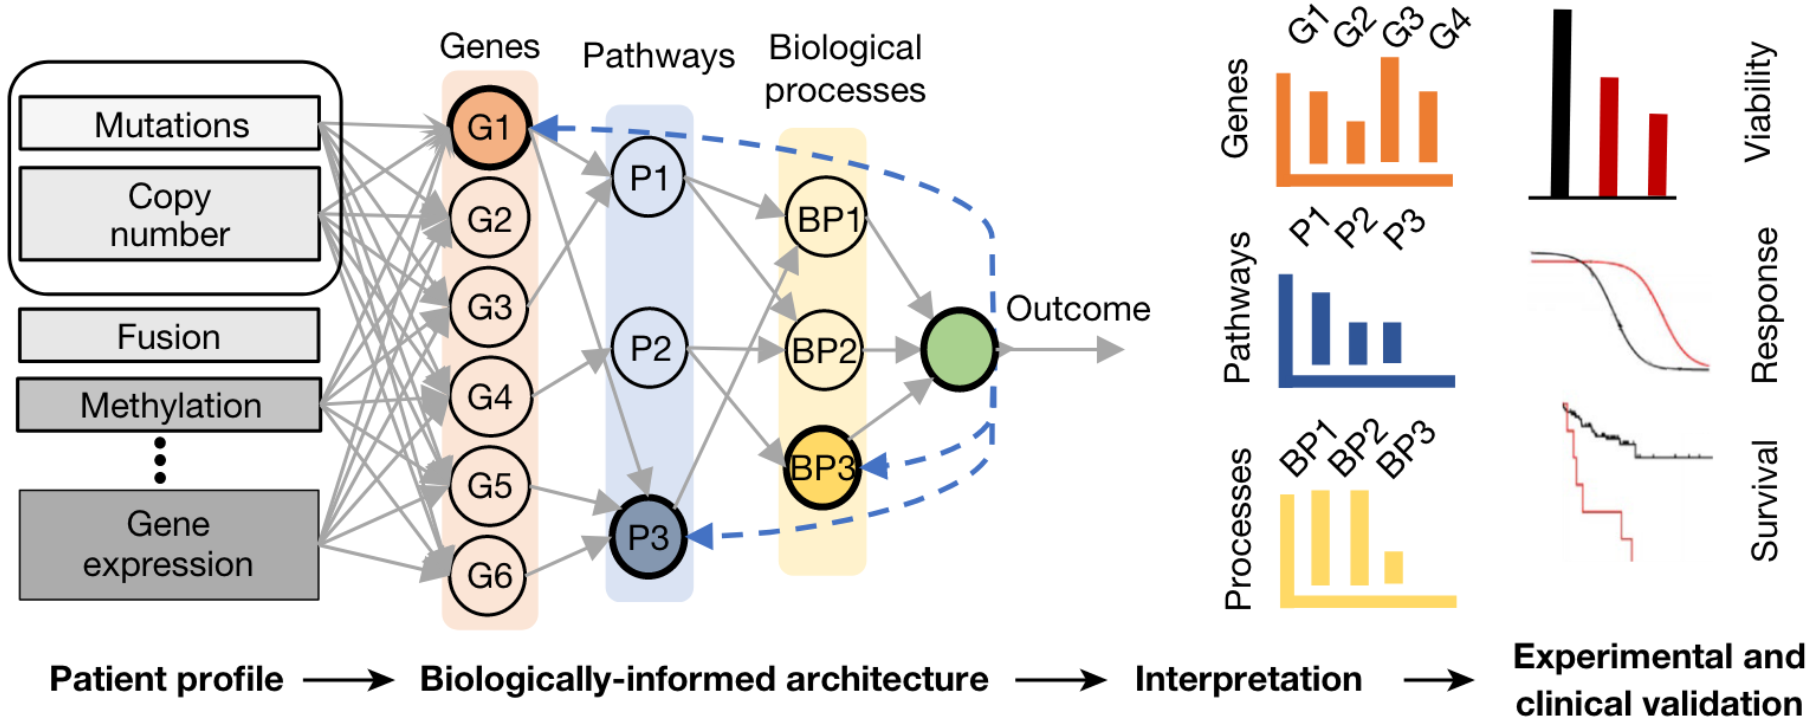
\includegraphics[width=\linewidth]{Figures/pnet_architecture.png}
    \caption{Architecture of the original P-NET neural network \cite{elmarakeby_biologically_2021} informed by the Reactome database. The number of nodes in the first layer corresponds to the number of genes in the Reactome database. These genes code for proteins, pathways and biological processes.}
    \label{fig:1}
\end{figure}

While the default first layer, which represents genes contains 14657 neurons, the biologically informed nature of P-NET has a reduced training speed over a fully connected network as the reduced number of connections results in fine-tuning of a gene set by only considering sub-graphs of the original network without entropy loss. The biologically informed nature of P-NET is automatically interpretable as each neuron is either a gene, pathway or a process.

\begin{figure}
    \centering
    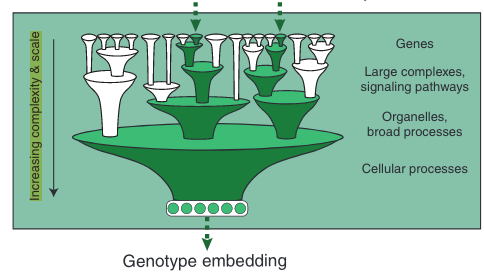
\includegraphics[width=\linewidth]{Figures/drugcell_architecture.png}
    \caption{DrugCell's \cite{kuenzi_predicting_2020} architecture, it is analogous to Reactome but the genes, biological processes and pathways are constructed independently and may not overlap.}
    \label{fig:2}
\end{figure}

\subsection{Regularisation}
Despite the sparse network the model is still prone to over-fitting. To prevent this we employ $\mathtt{L2}$ regularisation. This consists of adding a penalty term to the loss function:
\begin{equation}
    L_{L2} = \lambda \times \sum ||w||^2,
\end{equation}
for all the model weights $w$. This term will push the model towards smaller weights (or thus a simpler model). This term is characterised by the regularisation parameter $\lambda$, too small a value will lead to model overfitting, while too large can cause the weights to diverging to 0. In this case the model will not predict any variablility and instead predict for all outputs the mean of the training data.
\subsection{Transfer learning}
\subsection{Cross-validation and hyperparameter tuning}
Due to the very small available datasets we found the performance of a given model can vary significantly based on the test splitting of the data. In addition, the performance can vary based on the random seeds used in the stochastic minimization of the loss function. We also found that the performance can depend significantly on model hyper-parameters. If these are tuned to optimize the performance on a particular test splitting of the data this will result in an overly optimistic estimate of the performance when trained on unseen data.
\\ \indent To account for this we have developed a cross-validation procedure. This is used both to tune hyper-parameters and to make an unbiased estimate the model performance with a faithful uncertainty estimate. This procedure allows a fair comparison of different models.
\\ \indent We employ a procedure of nested-random-cross-validation \cite{}. A set of randomly chosen test datasets  are selected. In each case the remaining data is used to tune the model hyper-parameters. For this we use a grid search with random-cross validation. For every hyper-parameter set the data is is partitioned into a validation and a training set. The model training is run using the validation set to decide the early stopping of the training and to estimate the performance. This is then repeated a number of times to obtain an estimate of the mean performance and uncertainty for this hyper-parameter set. The hyper-parameter set with the best model performance are then used to train the model, with the performance judged on the test dataset. The distribution of this testing performance give an unbiased estimate of the model performance, with a reliable uncertainty estimate. This procedure is very computationally intensive and has been implemented using batch job submission in parallel on the Myriad cluster at UCL.
\\ \indent There are a number of hyper-parameters potentially affecting the model performance. For example the learning rate of the gradient descent and learning rate schedule, L2 regularization parameters, drop-out parameters etc (see more details in the previous section). 
These hyper-parameters can broadly be divided into two classes, those which control the minimization of the loss function and those which add some terms / modify it to prevent over-fitting. We found most of the hyper-parameters are correlated so focused on two for a optimization, the learning rate and the regularization parameter which are tuned using a grid search.  
\\ \indent Other model hyper-parameters are not formally optimized. To prevent bias these were set to reasonable values based on the scikit-learn and tensor-flow documentation and some initial tests on a single train / validation set. 
The choice of parameters is specified in Table \ref{tab:hyperpars}.
\begin{table}[]
    \centering
    \begin{tabular}{c|c}
       Hyperparameter  &  Value \\ \hline
       Regularisation parameter & Optimised - see text \\
       Learning rate  & Optimised - see text \\
      batch size  & 50 \\
      Early stopping patience &  - \\
     Maximum number of epochs &  - \\
     Optimiser &   - \\
     Loss weights &  \\
     Activation function & \\
    \end{tabular}
    \caption{The various hyperparameters used in training P-NET for radiation sensitivity.}
    \label{tab:hyperpars}
\end{table}
\\ \indent To asses model performance we compute the $R^2$ score defined as \cite{scikit-learn-docs}:
\begin{equation}
    R^2 = 1-\frac{\sum (y_i - \hat{y}_i)^2}{\sum_i (y_i - \bar{y})^2},
\end{equation}
where $y_i$ the value for data-point $i$, $\hat{y}_i$ is the associated prediction, while $\bar{y}$ is the mean of $y$. This gives a measure of the amount of variance in the outputs explained by the model.
%\input{method}

%---------------------------------------------------------------------


\section{Results}
\label{sec:results}
{\color{red}Toby: Here we could split up each of the 3 sub-projects but i think it would be more cohesive to just describe the results in parallel with the two network architectures}
\\
\subsection{Comparison of data types and architecture}
We train the model independently for three different data types (see \ref{sec:data}), gene-expression, copy number violation and mutations. This is performed for both the Reactome and Gene Ontology network architecture.
\\
{   \color{red}
Plots to include:
\begin{itemize}
    \item Example scatter plots ?
\item Performance for each of the 6 models?
\item Hyperparameter scan plot?
\end{itemize}}
\subsection{Transfer learning}
%\input{results}
%---------------------------------------------------------------------

\section{Conclusion}
\label{sec:conclusion}

\printbibliography
%\input{conclusion}
%---------------------------------------------------------------------

\end{document}
